\documentclass{article}
\usepackage[backend=biber,citestyle=ieee]{biblatex}
\usepackage[english]{babel}
% \usepackage[swedish]{babel}
\usepackage{graphicx}
\usepackage{csquotes}
\usepackage{float}
\usepackage{datetime}
\usepackage[title]{appendix}
% \usepackage{a4wide} 
\usepackage{amsmath}
\usepackage{subcaption}
\usepackage{textcomp}
\usepackage{gensymb}
\usepackage[font={small},margin={1cm}]{caption}

\usepackage{fancyhdr}   %page header
\pagestyle{fancy}

\usepackage[parfill]{parskip} %Line skip between paragraphs instead of indent

\usepackage{xcolor}
\usepackage{listings}

\definecolor{codegreen}{rgb}{0,0.6,0}
\definecolor{codegray}{rgb}{0.5,0.5,0.5}
\definecolor{codepurple}{rgb}{0.58,0,0.82}
\definecolor{backcolour}{rgb}{0.95,0.95,0.95}
\lstdefinestyle{mystyle}{
    backgroundcolor=\color{backcolour},   
    commentstyle=\color{codegreen},
    keywordstyle=\color{magenta},
    numberstyle=\tiny\color{codegray},
    stringstyle=\color{codepurple},
    basicstyle=\ttfamily\footnotesize,
    breakatwhitespace=false,         
    breaklines=true,                 
    captionpos=b,                    
    keepspaces=false,                 
    numbers=left,                    
    numbersep=5pt,                  
    showspaces=false,                
    showstringspaces=false,
    showtabs=false,                  
    tabsize=1
}
\lstset{style=mystyle}

%\addbibresource{sources.bib}

\newcommand{\getauthor}{Elias Berglin} %Author
\newcommand{\gettitle}{Labb 3} %Title
\newcommand\norm[1]{\left\lVert#1\right\rVert}

\newdateformat{daymonthyear}{\ordinal{DAY} \monthname[\THEMONTH] \THEYEAR} %Date

\title{\gettitle}
\author{\getauthor}

\date{\daymonthyear\today} %Remove for swedish date

\begin{document}

    % Title 
    \pagenumbering{gobble}
    \maketitle
    \newpage

    % Page header and footer
    \pagenumbering{arabic}
    \fancyhf{}
    \lhead{\getauthor}
    \rhead{\gettitle}
    \rfoot \thepage

    % Document starts here
    \section{Week 5}
    \subsection{Assignment 5}
    \subsubsection{Optical Flow}
    I used OpenCV's implementation for Optical Flow. This was originally used for videos but was adopted to be used with images instead. Coarse-to-fine algorithm improves our result on larger deltas by creating different layers of the image in different sizes. The smaller sizes helps the algorithm find features points. The itterations helps the algorithm to improve our results by correcting errors. In figure \ref{fig:flow-inputs} we can see the input images and in figure \ref{fig:flow-vectors} we can see the different results. We can see that the arrows correct them selves with more iterations and the points getting more accurate with more layers. The Python code can be found in appendix \ref{appendix:OF}

    \begin{figure}[H]
        \centering
        \begin{subfigure}{0.32\textwidth}
            \centering
            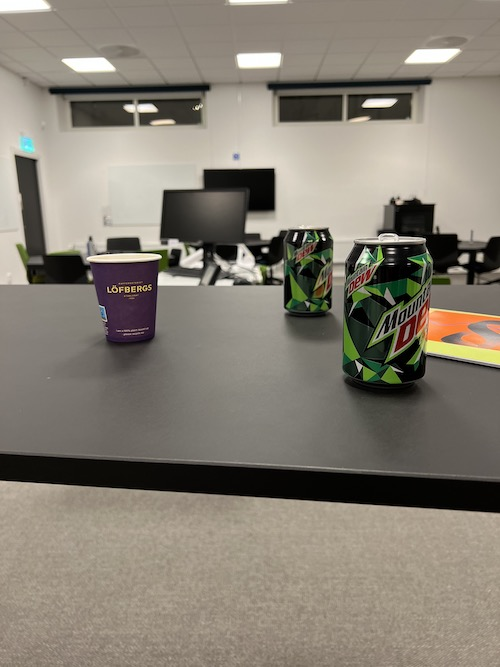
\includegraphics[width=1\textwidth]{im1.jpg}
            \caption{First image}
            \label{fig:sub:flow-first-frame}
        \end{subfigure}
        \begin{subfigure}{0.32\textwidth}
            \centering
            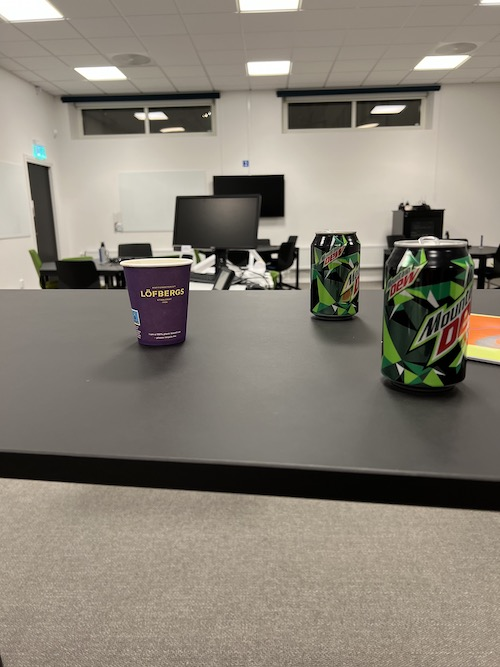
\includegraphics[width=1\textwidth]{im2.jpg}
            \caption{Second image}
            \label{fig:sub:flow-second-frame}
        \end{subfigure}  
        \begin{subfigure}{0.32\textwidth}
            \centering
            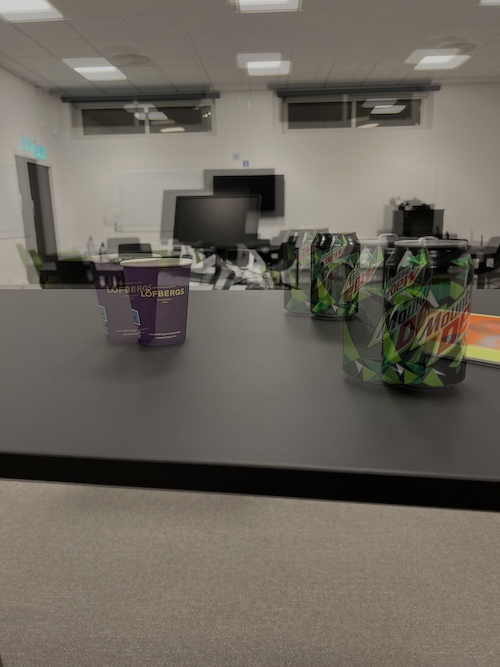
\includegraphics[width=1\textwidth]{combined.png}
            \caption{Images overlayed}
            \label{fig:sub:flow-combined}
        \end{subfigure} 
        \caption{The two input images for Optical Flow and the the images overlayed} 
        \label{fig:flow-inputs} 
    \end{figure}

    \begin{figure}[H]
        \centering
        \begin{subfigure}{0.48\textwidth}
            \centering
            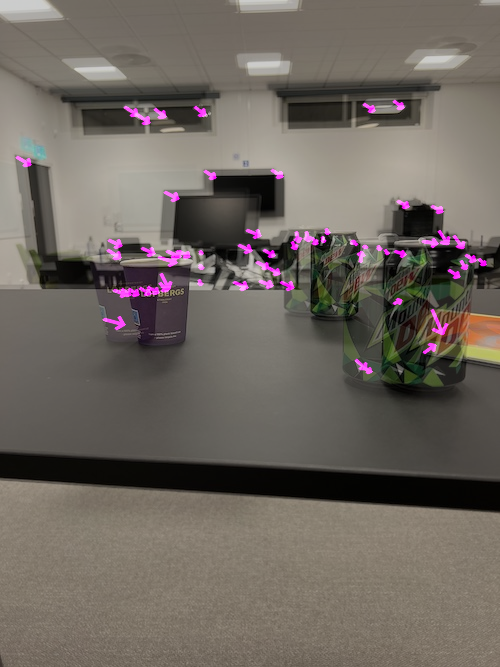
\includegraphics[width=1\textwidth]{2levels-2iterations.png}
            \caption{2 levels  and 2 iterations}
            \label{fig:sub:flow-low-it-no-pyr}
        \end{subfigure}
        \hspace{5px}
        \begin{subfigure}{0.48\textwidth}
            \centering
            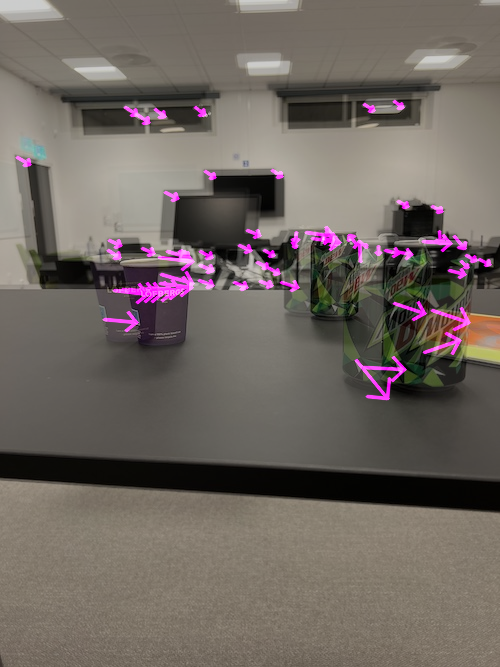
\includegraphics[width=1\textwidth]{2levels-10iterations.png}
            \caption{2 level and 10 iterations}
            \label{fig:sub:flow-low-it}
        \end{subfigure}  
        \begin{subfigure}{0.48\textwidth}
            \centering
            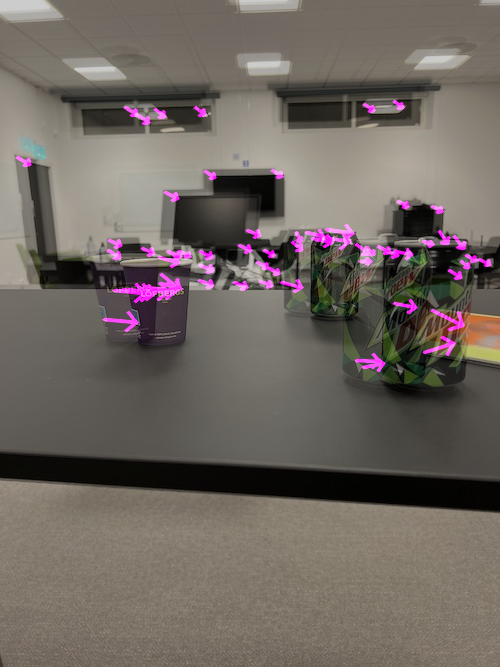
\includegraphics[width=1\textwidth]{3levels-2iterations.png}
            \caption{3 layers and 2 iterations}
            \label{fig:sub:flow-no-pyr}
        \end{subfigure}
        \hspace{5px}
        \begin{subfigure}{0.48\textwidth}
            \centering
            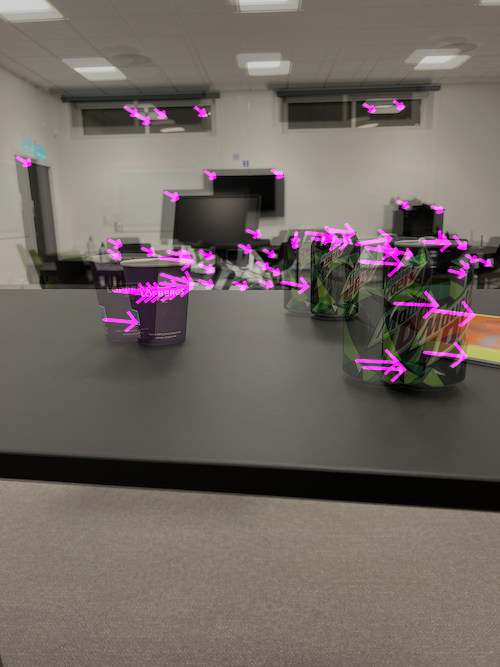
\includegraphics[width=1\textwidth]{3levels-10iterations.png}
            \caption{3 layers and 10 iterations}
            \label{fig:sub:flow}
        \end{subfigure}   
        \caption{Resulting vectors from Lucas-Kanade method with different amount of pyramids and iterations}
        \label{fig:flow-vectors}
    \end{figure}

    \subsubsection{K-means}
    The K-means function can be found in equation \ref{eq:kMeans}. This algorithm assumes that all of the datasets belong to a category $\mu$.
    \begin{equation}
        \label{eq:kMeans}
        \min_{\mu, y} \sum_i \norm{x_i - \mu_{y_i}}^2
    \end{equation}

    In figure \ref{fig:kMeansIter} we can se the different iterations. In figure \ref{fig:sub:k0} is the original data categorized. Then first iteratio in figure \ref{fig:sub:k1} and then when we compare that to \ref{fig:sub:k2} we see that nothing changes and thus our final categorized are decided.
    \begin{figure}[H]
        \centering
        \begin{subfigure}{0.32\textwidth}
            \centering
            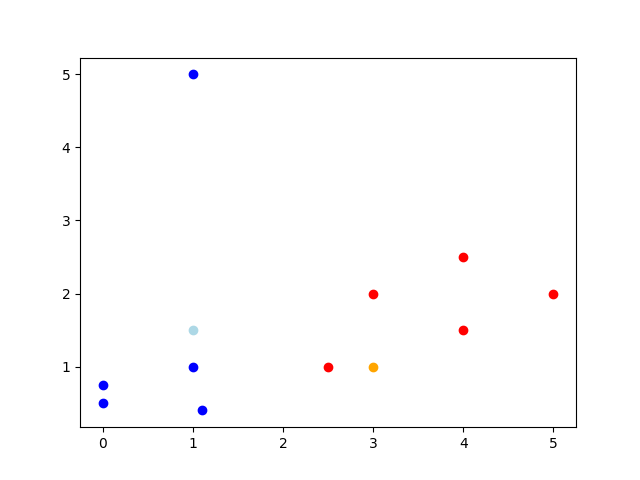
\includegraphics[width=1\textwidth]{k0.png}
            \caption{0 Iterations}
            \label{fig:sub:k0}
        \end{subfigure}
        \begin{subfigure}{0.32\textwidth}
            \centering
            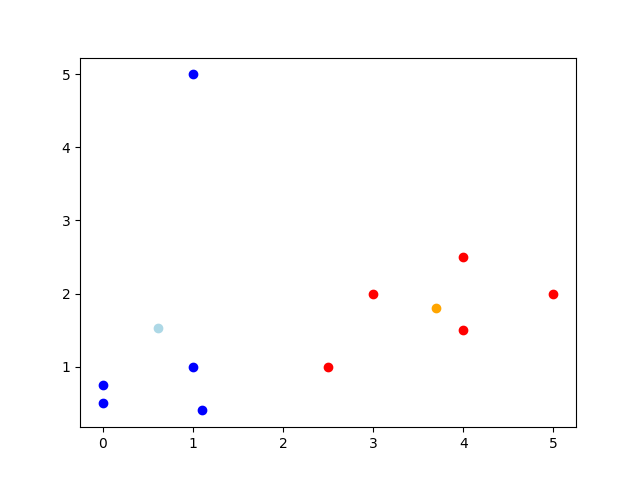
\includegraphics[width=1\textwidth]{k1.png}
            \caption{1 Iteration}
            \label{fig:sub:k1}
        \end{subfigure}  
        \begin{subfigure}{0.32\textwidth}
            \centering
            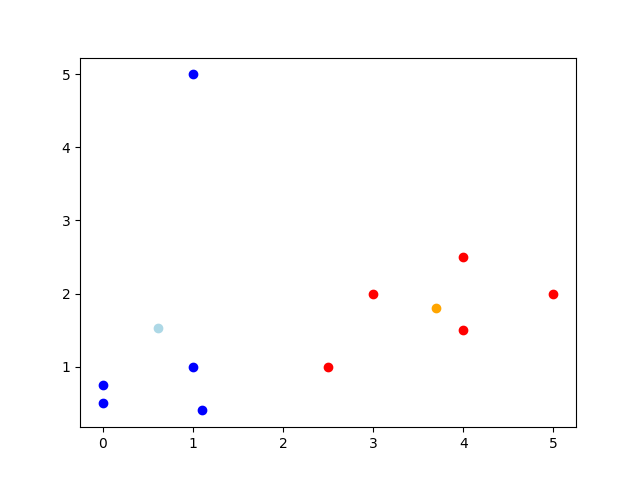
\includegraphics[width=1\textwidth]{k2.png}
            \caption{2 Iteration}
            \label{fig:sub:k2}
        \end{subfigure} 
        \caption{Iterations of K-means} 
        \label{fig:kMeansIter} 
    \end{figure}
    \subsubsection{Segmentation}


    % Sources
    %\newpage
    %\printbibliography

    % Appendices
    \newpage
    \begin{appendices}

        \section{Python code for optical flow}
        \label{appendix:OF}
        \begin{lstlisting}[language=Python]
import numpy as np
import cv2
import os

frame1 = cv2.imread("im1.jpg")
frame2 = cv2.imread("im2.jpg")

frame1g = cv2.cvtColor(frame1, cv2.COLOR_BGR2GRAY)
frame2g = cv2.cvtColor(frame2, cv2.COLOR_BGR2GRAY)

combined = cv2.addWeighted(frame1, 0.3, frame2, 0.5, 0)
cv2.imwrite("pyramid/combined.png", combined)

parameters = dict(maxCorners=100, qualityLevel=0.3, minDistance=7, blockSize=7)

p0 = cv2.goodFeaturesToTrack(frame1g, mask=None, **parameters)

maxLevels = [2,3]
maxIterations = [2, 10]

for level in maxLevels:
    print("On Max Level: ", level)
    for iter in maxIterations:
        OFparams = dict(
            winSize=(15, 15),
            maxLevel=level,
            criteria=(cv2.TERM_CRITERIA_EPS |
                      cv2.TERM_CRITERIA_COUNT, iter, 0.03),
        )
        p1, st, err = cv2.calcOpticalFlowPyrLK(
            frame1g, frame2g, p0, None, **OFparams)
        good_new = p1[st == 1]
        good_prev = p0[st == 1]

        arrows = np.zeros_like(combined)

        for i, (n, p) in enumerate(zip(good_new, good_prev)):
            nx, ny = n.ravel()
            px, py = p.ravel()

            nx = int(nx)
            ny = int(ny)
            px = int(px)
            py = int(py)

            arrows = cv2.arrowedLine(arrows, (px, py), (nx, ny), [
                                     255, 0, 255], 2, cv2.LINE_AA, tipLength=0.4)

            output = cv2.add(combined, arrows)
            if(not os.path.exists("pyramid/"+str(level))):
                os.mkdir("pyramid/"+str(level))
            outName = "pyramid/" + str(level)+"/" + \
                str(level) + "levels-" + str(iter)+"iterations.png"
            cv2.imwrite(outName, output)

        \end{lstlisting}

    \end{appendices}

\end{document}

% list with a,b,c
% \begin{enumerate}[label=(\alph*)]
%     \item 
% \end{enumerate}

% Centered figure with caption:
% \begin{figure}[H]
%     \centering
%     \includegraphics[width=1\textwidth]{%path} 
%     \caption{}
%     \label{fig:}
% \end{figure}

% Side by side figures:
% \begin{figure}[H]
%     \centering
%     \subfloat{{\includegraphics[width=0.46\textwidth]{%path} }}%
%     \qquad
%     \subfloat{{\includegraphics[width=0.46\textwidth]{%path} }}%
%     \caption{}
%     \label{fig:}
% \end{figure}

% Table with caption:
% \begin{table}[H]      
%     \begin{center}
%     \begin{tabular}{|c|c|} 
%         \hline
%         \textbf{} & \textbf{} \\\hline\hline
%          &  \\\hline 
%     \end{tabular}
%     \end{center}
%     \caption{}
%     \label{tab:}
% \end{table}

% Equation on multiple lines
% \begin{equation}
%    \begin{split}
%        x &= y \\
%        y &= z
%    \end{split}
% \end{equation}

% Code snippet
% \begin{lstlisting}%[language=]
%    //Code here
% \end{lstlisting}

% Code snippet from source file 
% \lstinputlisting[language=]{%path}
